\chapter{Spanner: Globally distributed database}

Spanner is a scalable, multi-version, globally-distributed, synchronously-replicated database.

\paragraph{External Consistency/Linearizability} If transaction T1 commits before another transaction T2 starts, then T1's commit timestamp is smaller than T2's


\section{Issues addressed} 
\begin{itemize}
    \item Wanted strong consistency (which via CAP theorem meant less availability)
    \item Wanted ACID transactions
    \item Wanted schema
    \item Spanner is an example of NewSQL (SQL like model, but scalability and performance)
    \item Built for F1 (important app for Google). Was MySQL cluster, had big problems of resharding (done manually) and schema migration.
    \item Wanted easy geodistribution (coping with whole datacentre failure)
    \item Wanted to automate the process of replication
\end{itemize}


\section{Main Ideas}
\begin{itemize}
    
    \item TrueTime API

    \item General-purpose transactions (ACID). Support different transaction types which are optimised e.g. non- blocking reads
    \begin{itemize}
        \item Write transactions guarantees 'external consistency' (strong form of consistency)
        \begin{itemize}
            \item Writes buffered. 
            \item Write locks acquired at commit time (when Paxos prepare is done). 
            \item But reducing availability for this (CAP) - block to wait out the uncertainty.
            \item Writes must initiate the Paxos protocol at the leader.
        \end{itemize}
        \item Reads access state directly from the underlying tablet at any replica that is sufficiently up-to-date.
        \item Read-Write - requires locks
        \item Read-Only - lock free
        \begin{itemize} 
            \item Requires declaration before start of transaction
            \item Reads information that is up-to-date
        \end{itemize}
        \item Snapshot-Read - read information from past by specifying timestamp or bound
        \begin{itemize}
            \item Lock free (non-blocking)
            \item Globally consistent
            \item Use specific timestamp from past or timestamp bound so that data until that point will be read
        \end{itemize}
    \end{itemize}

    \item Atomic schema changes

    \item Temporal database. Transaction serialization via global timestamps

    \item Schematised, semi-relational (tabular) data model
    \begin{itemize}
       \item SQL-like query interface
    \end{itemize}

    \item Data is versioned. Each version is automatically timestamped at commit time - while locks are held

    \item Data chunks - directory/bucket
    \begin{itemize}
        \item Unit of data movement and for defining replication properties
        \item Split into fragments
        \item Set of contiguous keys that share a common prefix.
        \item Locality encoded in to it - pick keys to get better locality
    \end{itemize}

    \item Shards data across many sets of Paxos groups
    \begin{itemize} 
        \item Want multiple groups to be able to partition data so you have smaller set of nodes to run Paxos on so its quicker. 
        \item Also, with multiple paxos groups they can have different ways of replication (nr replicas, location, etc). 
    \end{itemize} 

    \item Layering of how transactions are executed. 
    \begin{itemize} 
        \item If transaction can be done in one Paxos group then just run on that group. 
        \item When the transaction involves multiple paxos groups, then use the top layer (which uses strict two phase commit). This means users can do cross-row transactions 
    \end{itemize}

    \item Automatic resharding, rebalancing, failure response 

    \item Globally distributed for high availability and geographic locality. 

\end{itemize}

%---Truetime-----------------------------------------------------------
\subsection{TrueTime API} 
\begin{itemize} 
    \item Global timestamps 
    \item Exposes uncertainty in time and guarantees a bound on it 
    \item Timestamp as a range 
    \item Truetime timestamp getting is local, but these timestamps can be globally ordered (by reasoning about clock uncertainty/clock skew and waiting out the uncertainty to avoid overlapping timestamps) 
    \item TrueTime has masters that globally synchronize and decide on the global bound. 
    \item If network partition you lose the synchronization between the truetime masters. So must assume the clock skew increases over time, so over time the wait time will increase to where the system is very slow. (smaller clock uncertainty, larger throughput rate) 
    \item Uses GPS and atomic clocks to get accurate time. 
\end{itemize} 

\section{Additional points} 

\begin{wrapfigure}{R}{0.4\textwidth}
    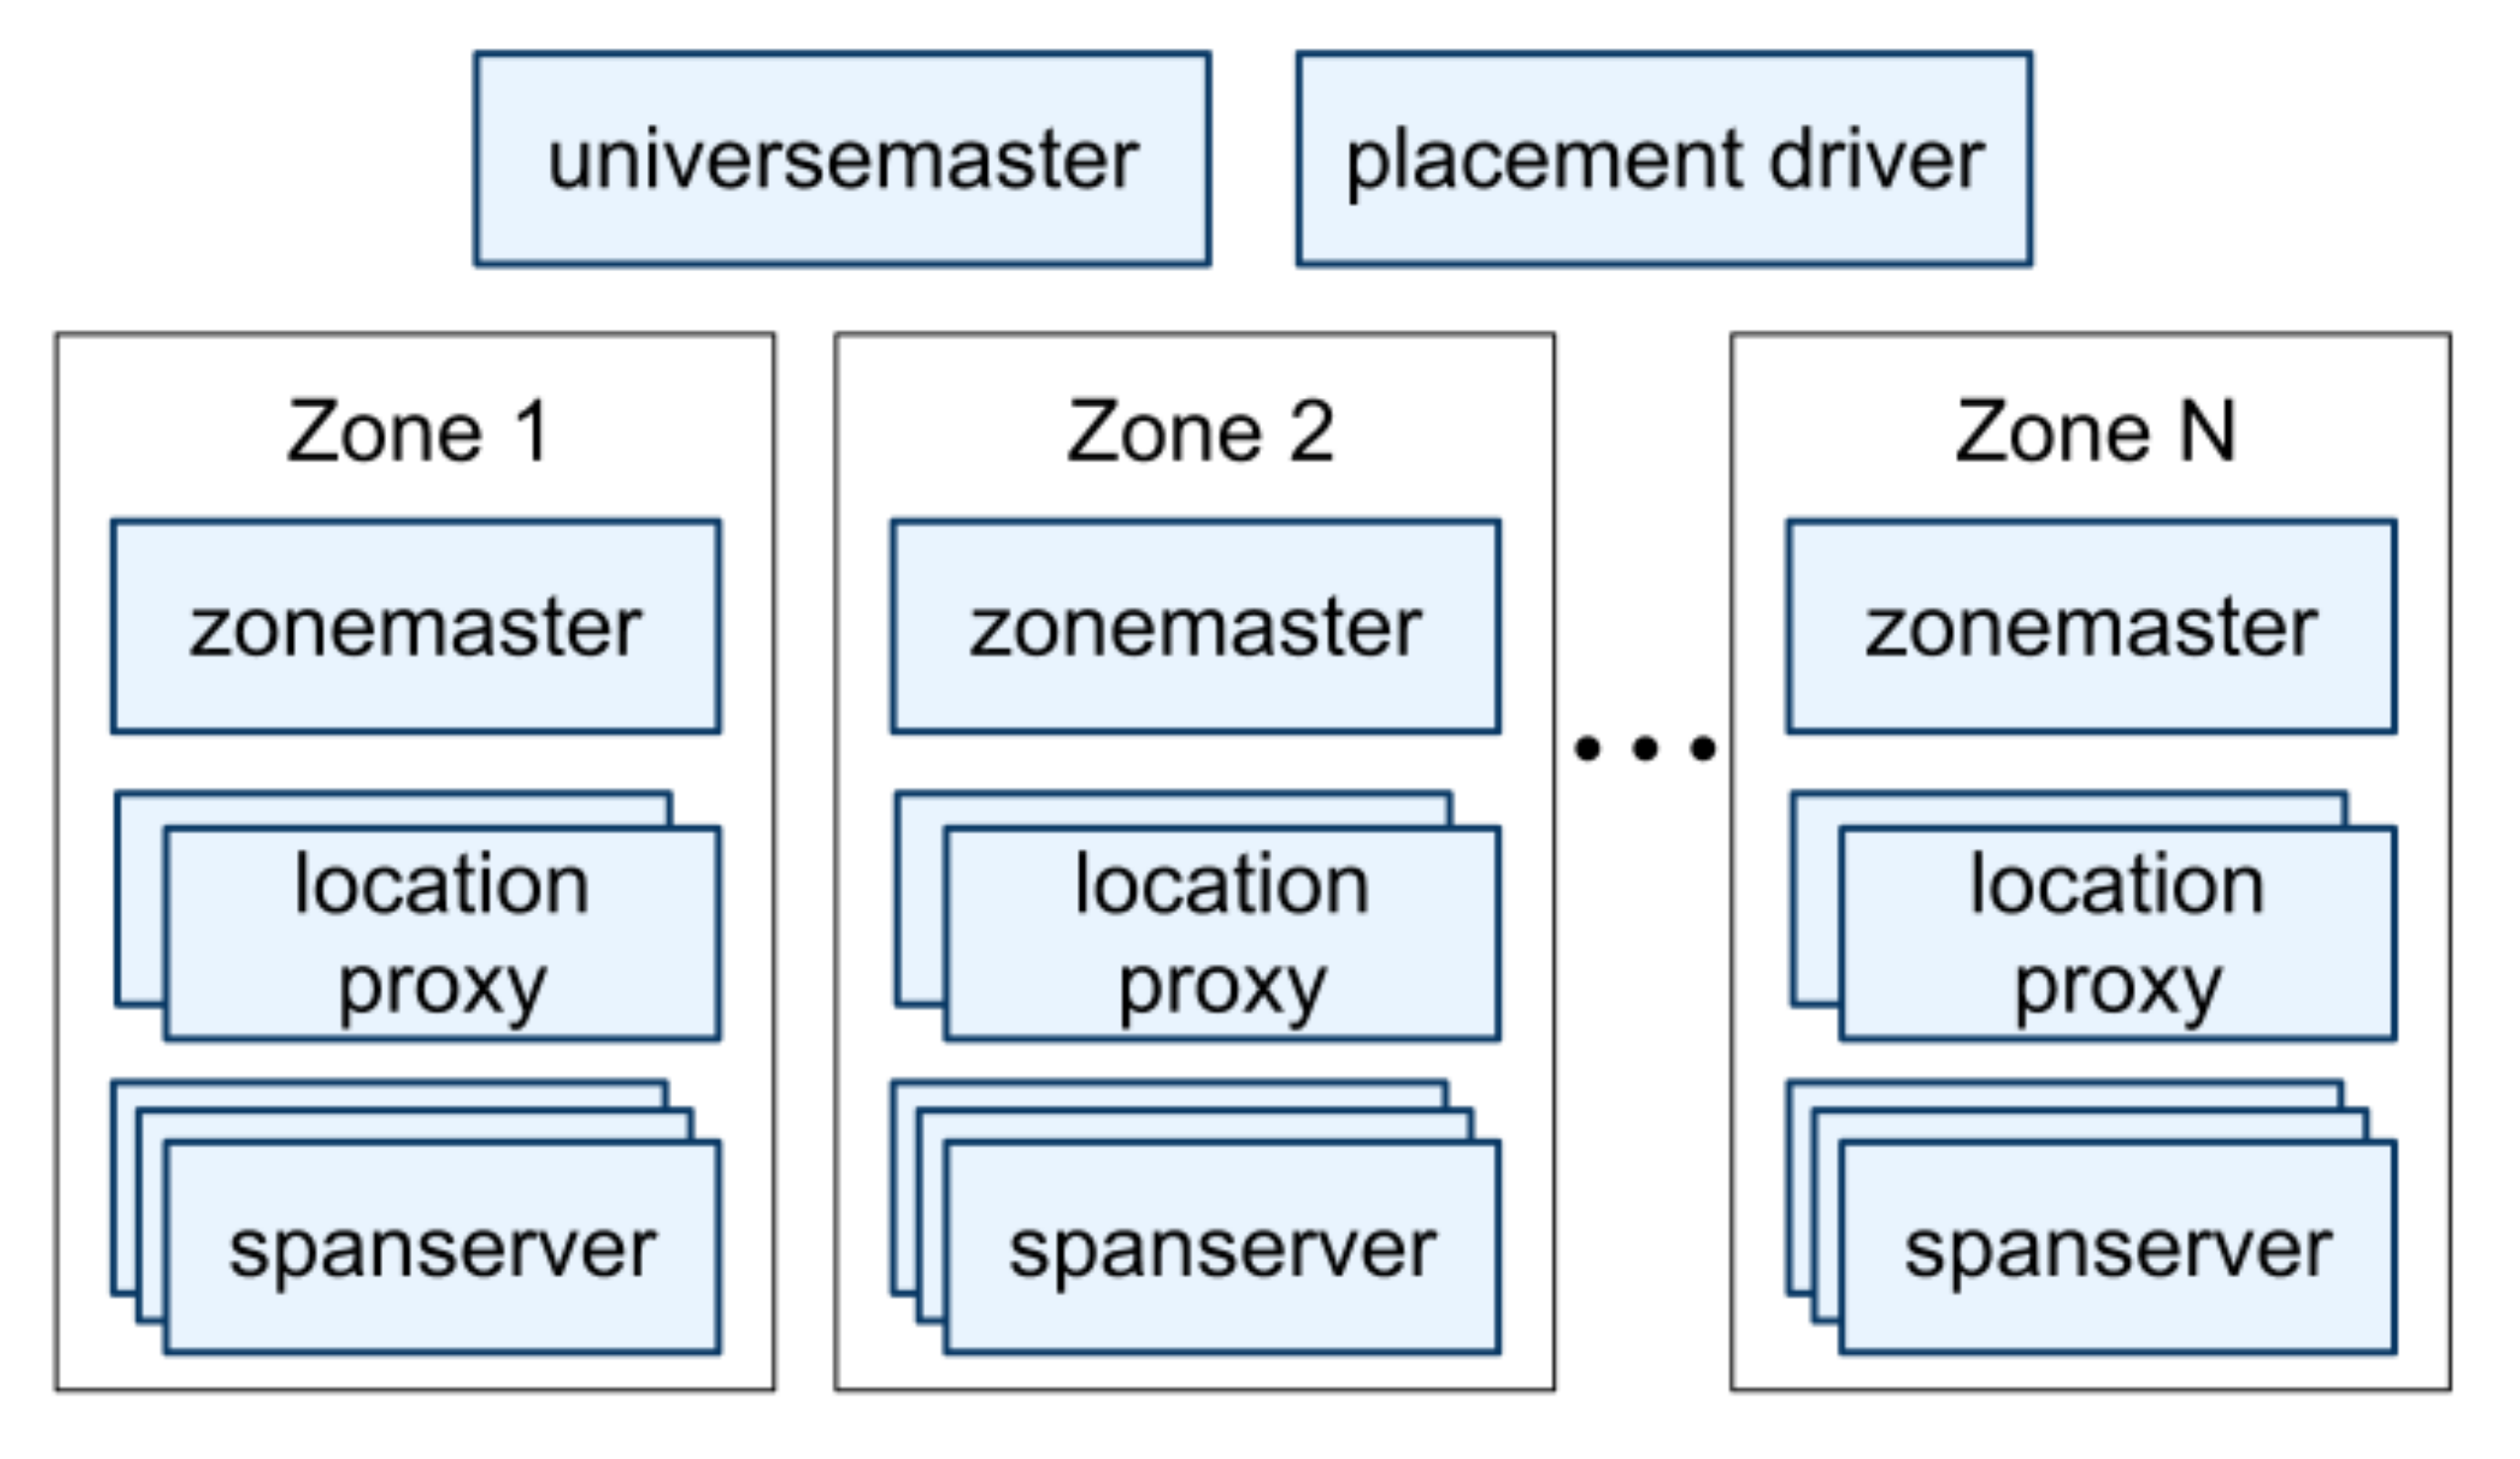
\includegraphics[width=0.39\textwidth]{img/spanner_archi.png}
\end{wrapfigure}

\begin{wrapfigure}{R}{0.4\textwidth}
    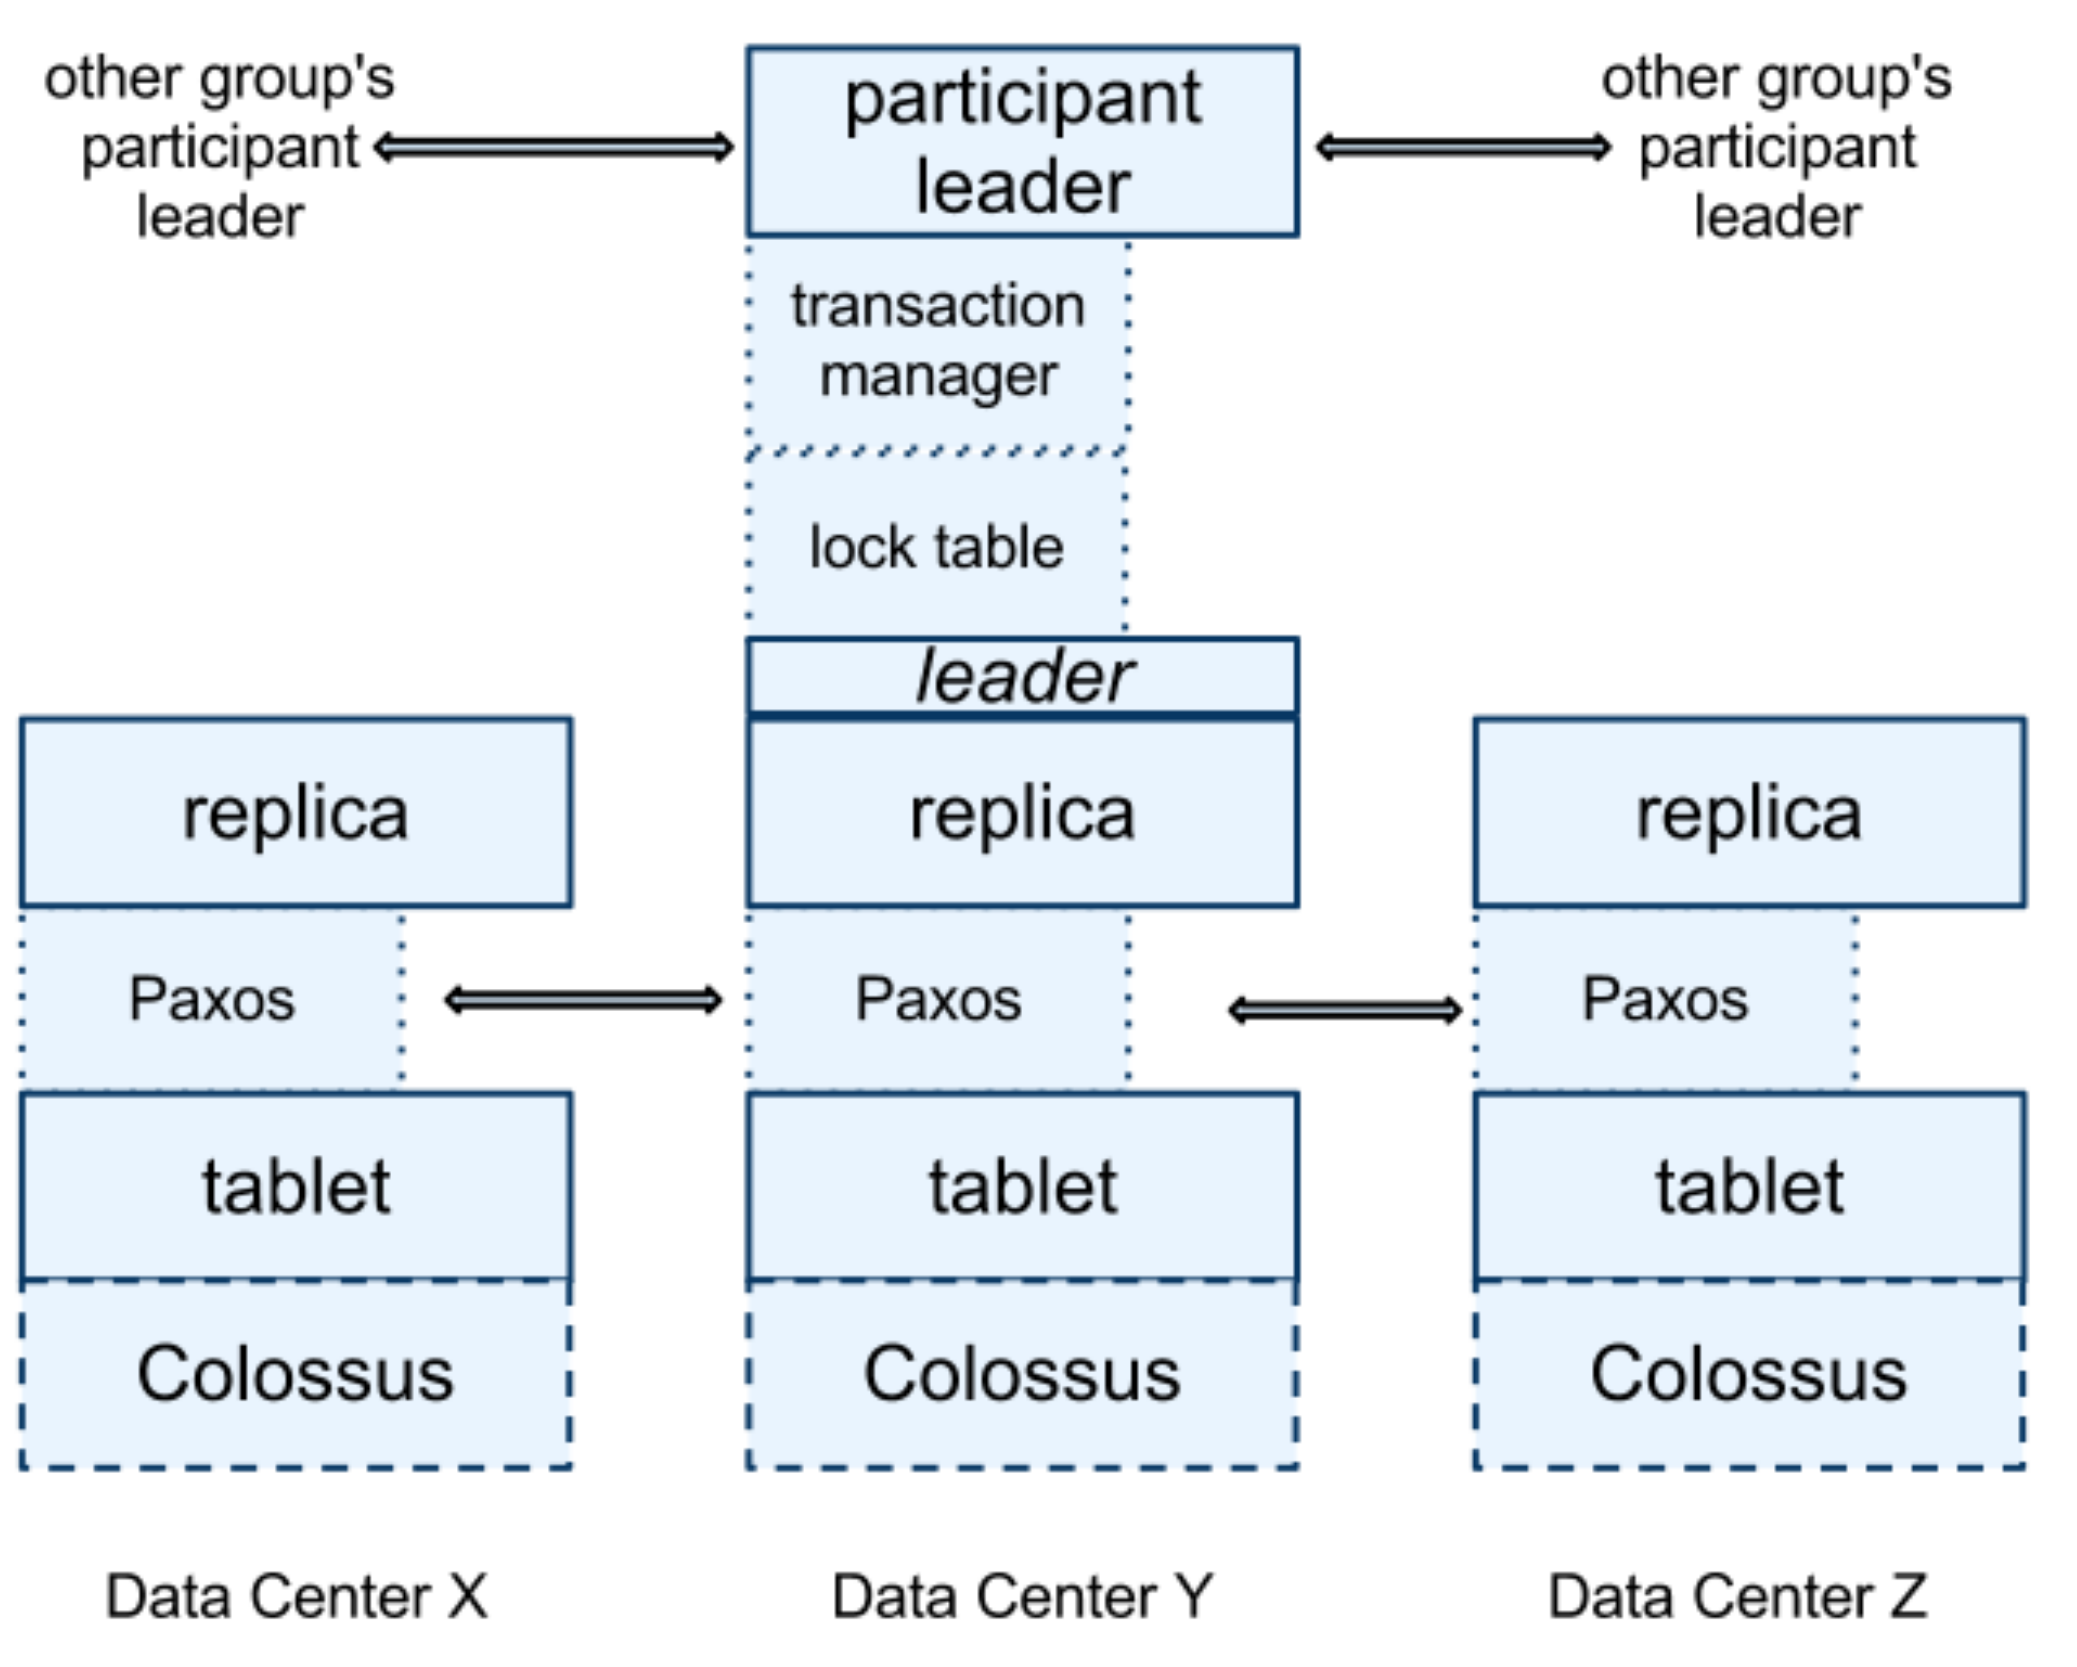
\includegraphics[width=0.39\textwidth]{img/spanner_system_diagram.png}
\end{wrapfigure}

\begin{itemize}
    \item Universe = Spanner deployment
    \item Zone = unit of administrative deployment; unit of physical isolation
    \item Zonemaster = assigns data to spanservers
    \item Spanservers = serve data to clients
    \item Location proxies = used by clients to locate the spanservers assigned to serve their data.
    \item Universe master = console that displays status info about all zones for interactive debugging
    \item Placement driver = handles automated movement of data across zones
    \item Tablet: data structure. Bag of key-value mappings (key, timestamp) to string. A container that may encapsulate multiple partitions of the row space, hence its possible to colocate mutiple directories that are frequently accessed together. Tablets are stored on top of the Colossus distributed file system. 
    \item Paxos state machine on each tablet.
    \item Long-lived leaders with time-based leader leases. If network partition happens, Paxos waits for 10 secs to get new leader. 
    \item Lock table at each replica that is a leader. Contains state for 2-phase locking.
    \item Transaction manager = used to support distributed transactions
    \item Participant leader = built on top of transaction manager; used when transactions involve multiple Paxos groups.
\end{itemize}

As the number of replicas increases, the latency to achieve a quorum becomes less sensitive to slowness at one slave replica.

Shorter lease times would reduce the effect of server deaths on availability, but would require gretaer amounts of lease-renewal network traffic.
